\chapter*{Proposition 33}



\begin{figure*}[ht]
    \begin{center}
    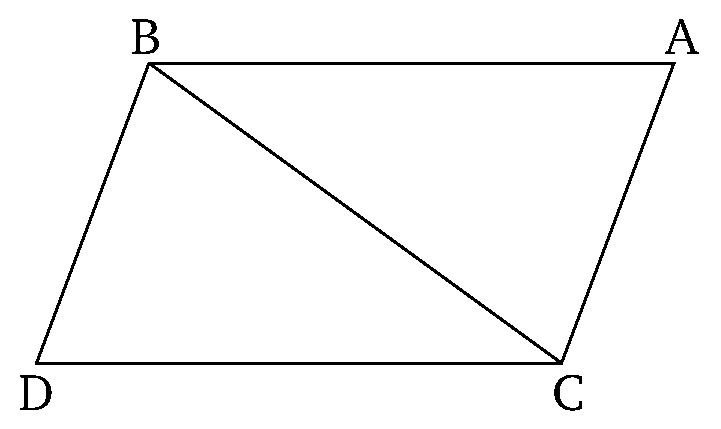
\includegraphics[width=0.5\linewidth]{figures/fig33e.eps}
    \label{fig:prop_33}
    \end{center}
\end{figure*}

Straight-lines joining equal and parallel (straight-lines) on the same sides
are themselves also equal and parallel.

Let $AB$ and $CD$ be equal and parallel (straight-lines), and let the
straight-lines $AC$ and $BD$ join them on the same sides. I say that $AC$
and $BD$ are also equal and parallel.

Let $BC$ have been joined. And since $AB$ is parallel to $CD$, and $BC$ has
fallen across them, the alternate angles $ABC$ and $BCD$ are equal to one another [Prop.~1.29]. And since $AB$ is equal to $CD$, and $BC$ is common,
the two (straight-lines) $AB$, $BC$ are equal to the two (straight-lines)
$DC$, $CB$.$^\dag$And the angle $ABC$ is equal to the angle $BCD$. Thus, the
base $AC$ is equal to the base $BD$, and triangle $ABC$ is equal to triangle
$DCB$$^\ddag$, and the remaining angles will be equal to the corresponding remaining
angles subtended by the equal sides [Prop.~1.4]. Thus,  angle $ACB$ 
is equal to $CBD$. Also, since the straight-line $BC$, (in) falling across the two
straight-lines $AC$ and $BD$, has made the alternate angles  ($ACB$ and $CBD$) equal to one another,
$AC$ is thus parallel to $BD$ [Prop.~1.27]. And ($AC$) was also shown (to be) equal
to ($BD$).

Thus, straight-lines joining equal and parallel (straight-lines) on the same sides
are  themselves also equal and parallel. (Which is) the very thing it was
required to show.


\section*{Commentary}

\begin{proposition}\label{proposition_33}\lean{Elements.Book1.proposition_33}\leanok
    If
\end{proposition}
\begin{proof}
    \uses{proposition_4,proposition_27,proposition_29}\leanok
\end{proof}
